% This file creates beamer slides for the paper Balboni et al 2024 FiFirm Adaptation in Production Networks: Evidence from Extreme Weather Events in Pakistan

\documentclass{beamer}

\usepackage[utf8]{inputenc} % Ensure proper encoding
\usepackage{graphicx} % For including images
\usepackage{hyperref} % For hyperlinks
\usepackage{amsmath,amsfonts,amssymb} % For mathematical symbols and equations

\setbeamertemplate{footline}[frame number] % Add page numbers to each slide

\begin{document}

\title{Firm Adaptation in Production Networks: Evidence from Extreme Weather Events in Pakistan}
\author{Clare Balboni, Johannes Boehm and Mazhar Waseem}

\institute{Muhammad Bashir, BSCD Lab}
\date{\today}

\frame{\titlepage}

\begin{frame}{Introduction}
\begin{itemize}
    \item Increased frequency and severity of extreme weather events are key
manifestations of projected climate change (IPCC 2021)
\item Firms impacted directly (Indaco et al 2021) and via exposure of supply
chain partners (Barrot \& Sauvagnat 2016, Carvalho et al 2021)
\item How costly these changes will be, and appropriate policy responses,
depend on whether and how firms and economic systems adapt
\item Firms' position in production networks may affect disaster exposure
via network nodes (supply partner firms) and links (supply routes)
\item Adaptive responses may involve complex network effects
\item Adjustments may reflect both direct disruptive impacts of disasters
and forward-looking decisions over future risk exposure
    
\end{itemize}

\end{frame}

\begin{frame}{Key Questions}
    \begin{itemize}
        \item Do firms adapt by changing production and network linkage
        decisions following natural disaster events?
        \begin{itemize}
            \item     What are the key margins of adaptation?
            \item What mechanisms underlie these adaptive responses?
            \item How important are adaptive decisions for aggregate outcomes?
        \end{itemize}
    
    \end{itemize}
\end{frame}

\begin{frame}{Approach}
    
\begin{itemize}
    \item Examine firm responses to floods in Pakistan and their network effects
    \item Impacts on firm operations and road transport
    \item Adaptive adjustments to mitigate future flood risk
    \item  Georeferenced microdata on firm networks from 2011-18
    Monthly data on near universe of firm-to-firm sales
    \item GPS tracker data on truck supply routes and disruptions
    Natural disaster and hazard exposure data
    \item Isolate forward-looking adaptive behavior from direct impacts using
    identification permitted by firm and route level flood disruption
\end{itemize}
\end{frame}

\begin{frame}{Results}
    \begin{itemize}
        \item Floods cause temporary disruption to firm operations and road usage
        \item Network effects key: 28\% firms flooded, 78\% experience supply partner flood, 46\% buyer-seller pairs experience transport route flood
        \item Persistent adaptive adjustments to own, supplier and route flooding
        \begin{itemize}
        \item Relocate to less flood-prone locations
        \item Diversify supplier base (cf Castro-Vincenzi 2022)
        \item Shift towards less flood-prone suppliers (cf Pankratz \& Schiller 2021)
        \item Shift towards suppliers reached via less flood-prone routes
        \item Responses reflect forward-looking actions to reduce vulnerability
        \item Identify changes in firm beliefs over flood risk
        \item Evidence consistent with persistent learning mechanism
    \end{itemize}
    
    \end{itemize}
    \end{frame}

\begin{frame}[allowframebreaks]{Thoughts}
    \label{thoughts}
\begin{itemize}
    \item    The adaptation is very quick? Does this mean something for adaptation channels? Could it be that same old suppliers are helping their purchasers source from other suppliers?
    \hyperlink{appendix}{\beamergotobutton{Diversification}}
    \item What is evidence in the literature in general on frictions to adaptation or just general optimizing frictions? Kleven and Waseem (2013) optimizing frictions? 
    \item  External Validity: Could it be that these Pakistani manufacturing firms are producing very basic goods and therefore it is easy to adjust? If you are producing more complex goods, it is harder to adjust as you would need very specific suppliers i.,e case of transistors in global supply chain disruptions?


 
    \item Forward looking adaptation hard to show empirically given data limitation but they do reasonably good job.


    \item They disentangle forward looking adaptation from mechanical adaptation by showing that they are also shifting away from other non-flooded suppliers who have flood risk? But can this also be mediated by the mechanical adaptation since now you employ different routes or you just choose a group of suppliers instead of each supplier separately? It is hard to show this since they do not observe goods supplied by a given supplier but just the PKR amount of purchases from that supplier. 
    \item The mechnical adaptation also has many channels such as it could be just that your old supplier cannot supply or that prices and economic environment has changed and hence you re-optimize? Importantly, they show firms respond to their own shocks and hence when your suppliers get a shock they also change their operations?
    \item People also asked how does a flood shock compare to other shocks such as financial shocks? 
    \item Similarly, where is this adjustment coming from? Are they trading off resilience to some other shocks in order to be more resilient to flood shocks? 
    \item Technically firms could also search for new buyers or customers in response to shocks to places where they make sales? They do not study this!
    \item Similarly, what are effects on the firms up the supply chains? Low power to study this!
    \item What is governmet's response in terms of investments in flood shock resilient infrastructure?
    \item It would be good to study characteristics of new destinations and new suppliers.    
    

\end{itemize}
\end{frame}

\begin{frame}[allowframebreaks]{Appendix}
    \label{appendix}
    \begin{figure}
        \centering
        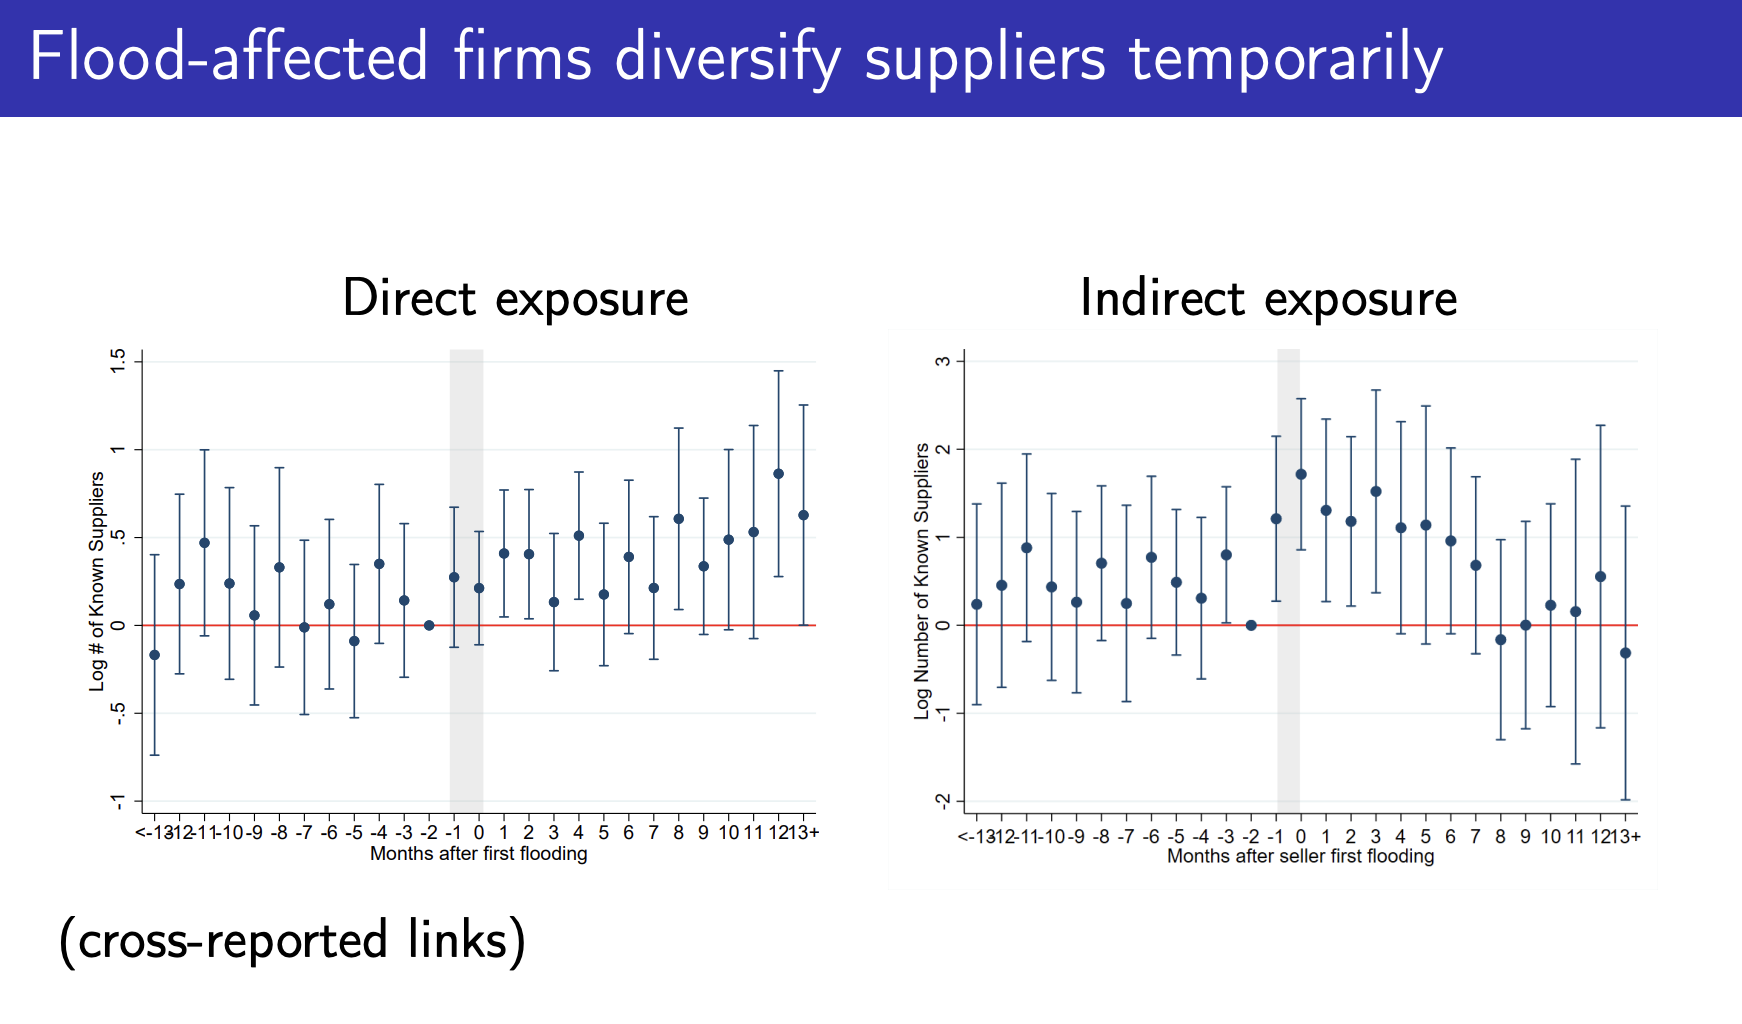
\includegraphics[width=0.8\textwidth]{F1.png}
        \label{fig:appendix1}
        \hyperlink{thoughts}{\beamerreturnbutton{Return}}  % Add this line
    \end{figure}

\begin{figure}
    \centering
    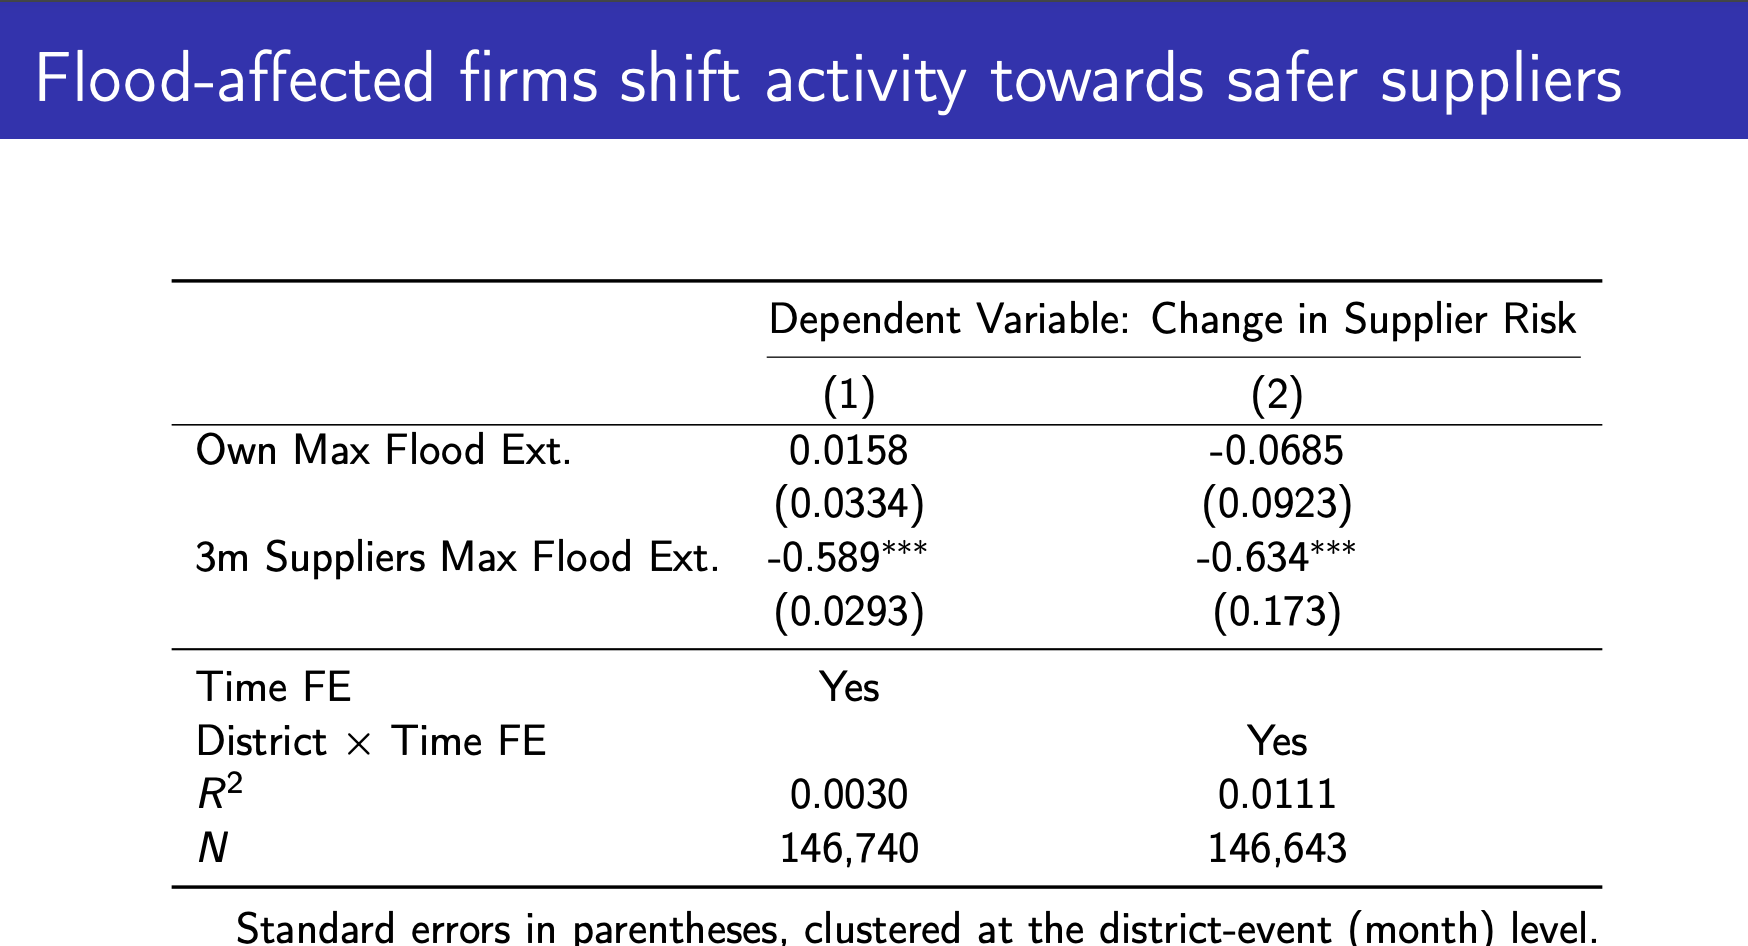
\includegraphics[width=0.8\textwidth]{F2.png}
    \label{fig:appendix2}
\end{figure}

    \hyperlink{thoughts}{\beamerreturnbutton{Return}}  % Add this line
\begin{figure}
    \centering
    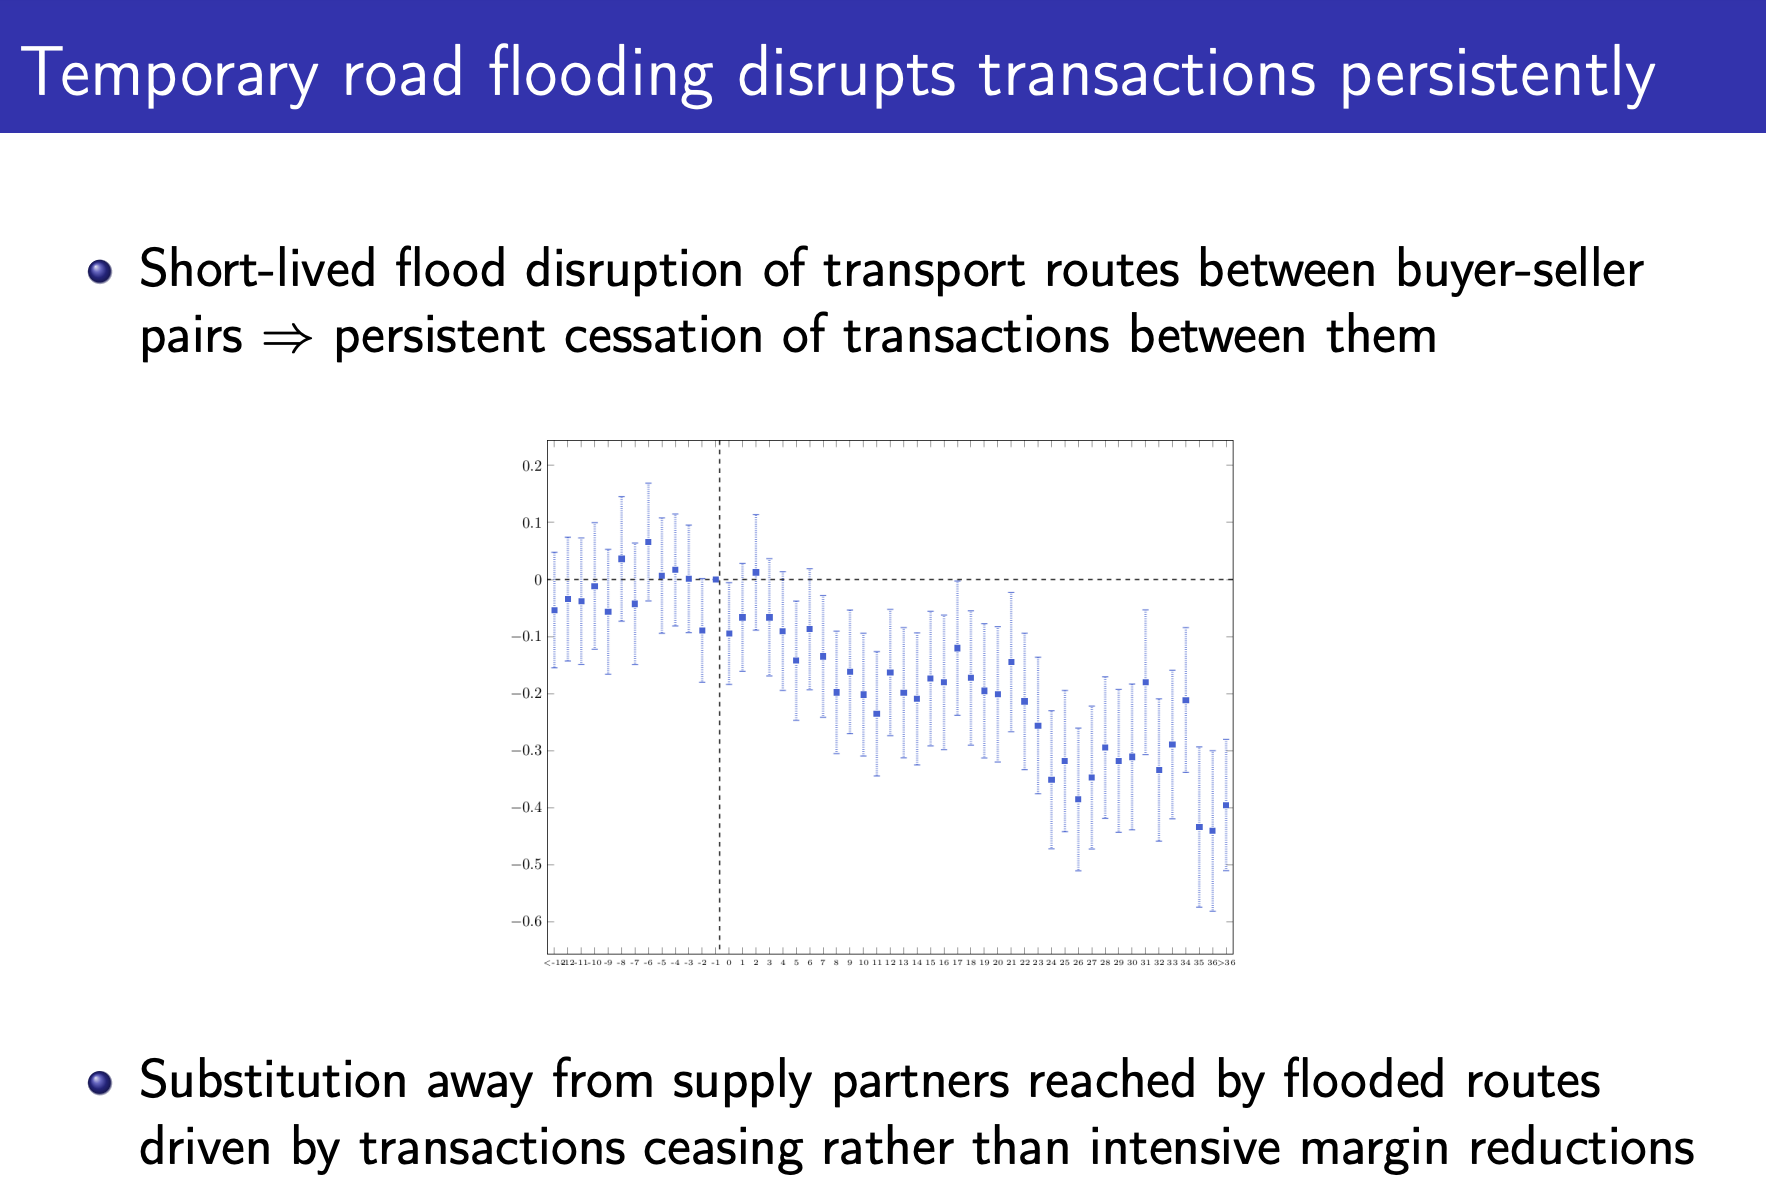
\includegraphics[width=0.8\textwidth]{F3.png}
    \label{fig:appendix3}
\end{figure}
\hyperlink{thoughts}{\beamerreturnbutton{Return}}  % Add this line

\end{frame}

\end{document}
